\section{Ecuación de la recta }
\subsection{Descripción del problema}
Dados dos puntos A y B, con coordenadas x1,y1 y x2,y2. Se regresara la ecuación de la recta y el ángulo interno que se forma entre el eje horizontal y la recta.
\subsection{Definición de solución}
En la ecuación de la recta si dos puntos distintos $P(x_{1},y_{1})$ y $Q(x_{2},y_{2})$ se ubican en la curva $y=f(x)$, la pendiente de la recta Secante que une los dos puntos es:

\begin{equation}
    m_{sec} = \frac{y_{1}-y_{2}}{x_{1}-x_{2}} = \frac{f(x_{1})-f(x_{2})}{x_{1}-x_{2}}
\end{equation}

Para identificar la intersección en el eje vertical se utiliza cualquiera de los dos puntos para este caso se utilizo $P(x_{1},y_{1})$ de la siguiente forma: 
\begin{equation}
    b = y_{1} - m_{sec} * x_{1} 
\end{equation}

\begin{figure}[h!]
    \centerline{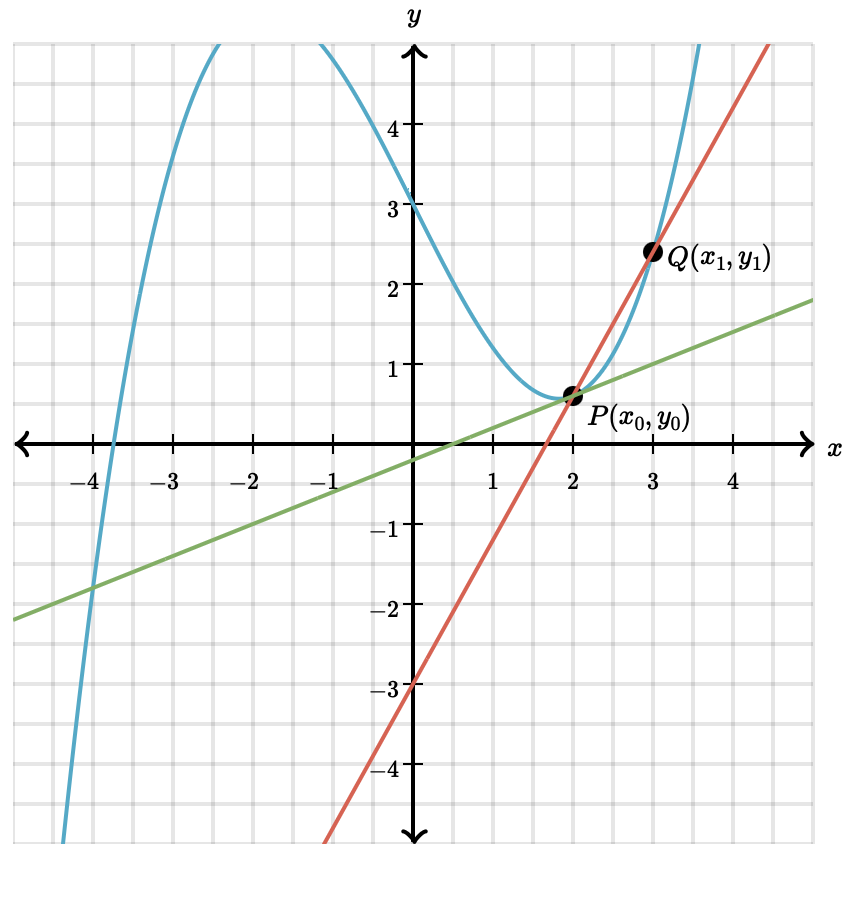
\includegraphics[width = 6cm]{Latex-imágenes/GraficaEcuacionRecta.png}}
    \caption{Gráfica de la ecuación de la recta}
    \label{fig}
\end{figure}

Utilizando este método, puedes encontrar la ecuación de la recta a partir de dos puntos dados. Recuerda que si los dos puntos son idénticos, la recta sera una linea vertical\cite{articuloRecta}
\section{Ecuación para el ángulo de la recta}
Y para calcular el ángulo de dicha pendiente se usa: 

\begin{equation}
    \sphericalangle=\arctan(m)
\end{equation}
\subsection{Diseño de solución}
Asignar valores de usuarios a la variables de la ecuación de la recta, calcular la pendiente de la recta, calcular el ángulo interno entre la recta y el eje horizontal e imprimir la ecuación de la recta y el ángulo interno
\subsection{Desarollo de la solución}
\begin{javaCode}
 
        // Asignar valores de usuario a las variables de la ecuación de la recta
        double x1 = Double.parseDouble(punto1[0].trim());
        double y1 = Double.parseDouble(punto1[1].trim());

        double x2 = Double.parseDouble(punto2[0].trim());
        double y2 = Double.parseDouble(punto2[1].trim());

        // Calcular la pendiente de la recta
        double m = (y2 - y1) / (x2 - x1);

        // Calcular el ángulo interno α entre la recta y el eje horizontal
        double alpha = Math.toDegrees(Math.atan(m));

        // Imprimir la ecuación de la recta y el ángulo interno α
        System.out.println("Ecuación de la recta: y = " + m + "x + " + (y1 - m * x1));
        System.out.println("Ángulo interno α: " + alpha + " grados");
    }
}
\end{javaCode}
\subsection{Depuración y pruebas}
\begin{tabular}{|c|c|c||c||c||c|}
  \hline
  Corrida & X1Y1 & X2Y2 & Recta & Ángulo \\
  \hline
  1 & 1,6 & 3,5 & y=-0.5x+6.5 & 116° \\
  \hline
  2 & 3,7 & 2,0 & y=7.0x+-14.0 & 8.130° \\
  \hline
  3 & 23 & 47 & No valido & No valido \\
  \hline
  
\end{tabular}
